\begin{center}
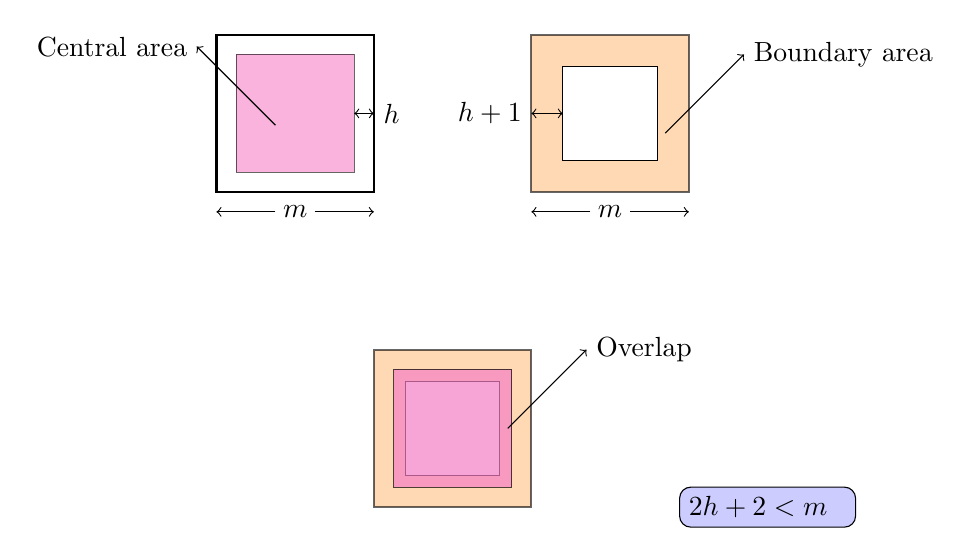
\begin{tikzpicture}

    % First square: Central area highlighted
    \draw[thick] (0, 2) rectangle ++(2, 2);
    \draw[fill=magenta!50, opacity = 0.6] (0.25, 2.25) rectangle ++(1.5, 1.5);
    \draw[->] (0.75, 2.85) -- ++(-1, 1) node[left] {Central area};
    \draw[->] (0.75, 1.75) -- (0, 1.75) ;
    \draw[->] (1.25, 1.75) -- (2, 1.75) ;
    \draw[<->] (1.75, 3) -- ++(0.25, 0) node[right] {$h$};
    \node at (1,1.75) {$m$};

    % Second square: Boundary area highlighted
    \draw[thick,fill=orange!50, opacity = 0.6] (4, 2) rectangle ++(2, 2);
    \draw[fill=white] (4.4, 2.4) rectangle ++(1.2, 1.2);
    \draw[->] (5.7, 2.75) -- ++(1, 1) node[right] {Boundary area};
    \draw[->] (4.75, 1.75) -- (4, 1.75) ;
    \draw[->] (5.25, 1.75) -- (6, 1.75) ;
    \draw[<->] (4.4, 3) -- ++(-0.4, 0) node[left] {$h +1$};
    \node at (5,1.75) {$m$};

    % Third square: Both areas highlighted
    \draw[thick, fill=orange!50, opacity = 0.6] (2, -2) rectangle ++(2, 2);
    \draw[fill=white] (2.4, -1.6) rectangle ++(1.2, 1.2);
    \draw[fill=magenta!50, opacity=0.7] (2.25, -1.75) rectangle ++(1.5, 1.5);
    \draw[->] (3.7, -1) -- ++(1, 1) node[right] {Overlap};

    \node[draw, fill=blue!20, text width=2cm, rounded corners] at (7, -2) {
           $2h + 2 < m$
            };
    

\end{tikzpicture}
\end{center}